% Generated by extension/synthesis/make_assets.py. Do not edit.
\definecolor{propcol}{HTML}{217D91}
\definecolor{pairedcol}{HTML}{5D6670}
\definecolor{semicol}{HTML}{C9803A}
\definecolor{champcol}{HTML}{8E4B8C}
\definecolor{ridgecol}{HTML}{9AA3AB}
\definecolor{meancol}{HTML}{A64442}
\definecolor{sitecol}{HTML}{6A8FB3}
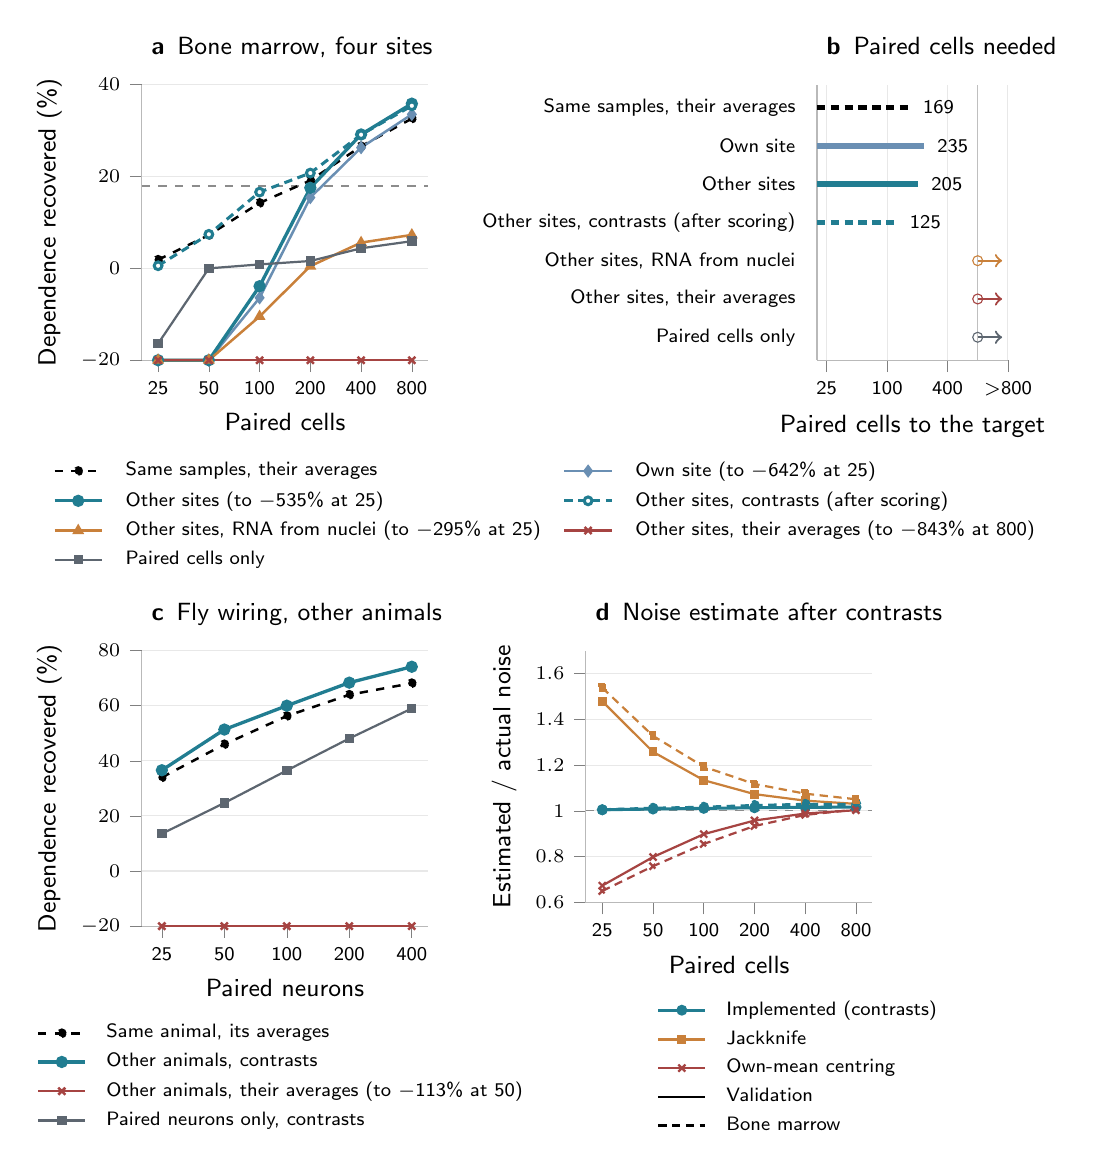
\begin{tikzpicture}[font=\sffamily]
\begin{axis}[name=a,scale only axis,width=.3\textwidth,height=3.5cm,xmode=log,log basis x=2,
 xmin=20,xmax=1000,ymin=-20,ymax=40,xtick={25,50,100,200,400,800},xticklabels={25,50,100,200,400,800},ytick={-20,0,20,40},
 xlabel={Paired cells},ylabel={Dependence recovered (\%)},
 title={\textbf{a}\enspace Bone marrow, four sites},
 axis x line*=bottom,axis y line*=left,tick align=outside,ymajorgrids=true,grid style={gray!18},axis line style={gray!55},tick label style={font=\sffamily\scriptsize},label style={font=\sffamily\small},clip=false,title style={font=\sffamily\small,at={(0,1)},anchor=base west,yshift=5pt}]
\draw[dashed,black!45] (axis cs:20,17.93) -- (axis cs:1000,17.93);
\addplot[color=black,line width=.9pt,dashed,mark=*,mark size=1.3pt] coordinates { (25,1.87) (50,7.25) (100,14.24) (200,19.13) (400,26.57) (800,32.61) };
\addplot[color=sitecol,line width=.9pt,mark=diamond*,mark size=1.7pt] coordinates { (25,-20.00) (50,-20.00) (100,-6.41) (200,15.42) (400,26.29) (800,33.52) };
\addplot[color=propcol,line width=1.2pt,mark=*,mark size=1.6pt] coordinates { (25,-20.00) (50,-20.00) (100,-3.89) (200,17.54) (400,29.15) (800,35.86) };
\addplot[color=propcol,line width=1.1pt,densely dashed,mark=*,mark size=1.4pt,mark options={solid,fill=white}] coordinates { (25,0.57) (50,7.41) (100,16.60) (200,20.75) (400,29.10) (800,35.40) };
\addplot[color=semicol,line width=.9pt,mark=triangle*,mark size=1.6pt] coordinates { (25,-20.00) (50,-20.00) (100,-10.47) (200,0.48) (400,5.61) (800,7.28) };
\addplot[color=meancol,line width=.9pt,mark=x,mark size=1.8pt] coordinates { (25,-20.00) (50,-20.00) (100,-20.00) (200,-20.00) (400,-20.00) (800,-20.00) };
\addplot[color=pairedcol,line width=.8pt,mark=square*,mark size=1.3pt] coordinates { (25,-16.39) (50,0.00) (100,0.86) (200,1.60) (400,4.37) (800,5.92) };
\end{axis}
\begin{axis}[at={(a.outer north east)},anchor=outer north west,xshift=.4cm,name=b,scale only axis,width=.2\textwidth,height=3.5cm,xmode=log,log basis x=2,
 xmin=20,xmax=1600,ymin=.4,ymax=7.6,xtick={25,100,400,1600},xticklabels={25,100,400,$>$800},
 ytick={1,2,3,4,5,6,7},
 yticklabels={{Paired cells only},{Other sites, their averages},{Other sites, RNA from nuclei},{Other sites, contrasts (after scoring)},{Other sites},{Own site},{Same samples, their averages}},
 xlabel={Paired cells to the target},
 title={\textbf{b}\enspace Paired cells needed},
 axis x line*=bottom,axis y line*=left,tick align=outside,xmajorgrids=true,grid style={gray!18},axis line style={gray!55},tick label style={font=\sffamily\scriptsize},label style={font=\sffamily\small},clip=false,title style={font=\sffamily\small,at={(0,1)},anchor=base west,yshift=5pt},y tick style={draw=none}]
\draw[black!25] (axis cs:800,.4) -- (axis cs:800,7.6);
\draw[->,color=pairedcol,line width=.8pt] (axis cs:800,1) -- (axis cs:1400,1);
\addplot[only marks,mark=o,mark size=1.8pt,color=pairedcol] coordinates { (800,1) };
\draw[->,color=meancol,line width=.8pt] (axis cs:800,2) -- (axis cs:1400,2);
\addplot[only marks,mark=o,mark size=1.8pt,color=meancol] coordinates { (800,2) };
\draw[->,color=semicol,line width=.8pt] (axis cs:800,3) -- (axis cs:1400,3);
\addplot[only marks,mark=o,mark size=1.8pt,color=semicol] coordinates { (800,3) };
\draw[color=propcol,line width=1.6pt,densely dashed] (axis cs:20,4) -- (axis cs:124.9,4);
\node[font=\sffamily\scriptsize,anchor=west] at (axis cs:134.9,4) {125};
\draw[color=propcol,line width=2.4pt] (axis cs:20,5) -- (axis cs:204.7,5);
\node[font=\sffamily\scriptsize,anchor=west] at (axis cs:221.1,5) {205};
\draw[color=sitecol,line width=2.4pt] (axis cs:20,6) -- (axis cs:234.7,6);
\node[font=\sffamily\scriptsize,anchor=west] at (axis cs:253.5,6) {235};
\draw[color=black,line width=1.6pt,densely dashed] (axis cs:20,7) -- (axis cs:168.7,7);
\node[font=\sffamily\scriptsize,anchor=west] at (axis cs:182.2,7) {169};
\end{axis}
\path (a.outer south west) -- (b.outer south east) coordinate[pos=.5] (legab);
\begin{axis}[hide axis,scale only axis,width=1pt,height=1pt,xmin=0,xmax=1,ymin=0,ymax=1,at={(legab)},anchor=north,yshift=-2pt,legend style={draw=none,font=\sffamily\scriptsize,at={(0.5,0.5)},anchor=north,legend columns=2,column sep=6pt,cells={anchor=west}}]
\addlegendimage{color=black,line width=.9pt,dashed,mark=*,mark size=1.3pt}
\addlegendentry{Same samples, their averages}
\addlegendimage{color=sitecol,line width=.9pt,mark=diamond*,mark size=1.7pt}
\addlegendentry{Own site (to \ensuremath{-}642\% at 25)}
\addlegendimage{color=propcol,line width=1.2pt,mark=*,mark size=1.6pt}
\addlegendentry{Other sites (to \ensuremath{-}535\% at 25)}
\addlegendimage{color=propcol,line width=1.1pt,densely dashed,mark=*,mark size=1.4pt,mark options={solid,fill=white}}
\addlegendentry{Other sites, contrasts (after scoring)}
\addlegendimage{color=semicol,line width=.9pt,mark=triangle*,mark size=1.6pt}
\addlegendentry{Other sites, RNA from nuclei (to \ensuremath{-}295\% at 25)}
\addlegendimage{color=meancol,line width=.9pt,mark=x,mark size=1.8pt}
\addlegendentry{Other sites, their averages (to \ensuremath{-}843\% at 800)}
\addlegendimage{color=pairedcol,line width=.8pt,mark=square*,mark size=1.3pt}
\addlegendentry{Paired cells only}
\end{axis}
\begin{axis}[at={(a.outer south west)},anchor=outer north west,yshift=-1.95cm,name=c,scale only axis,width=.3\textwidth,height=3.5cm,xmode=log,log basis x=2,
 xmin=20,xmax=480,ymin=-20,ymax=80,xtick={25,50,100,200,400},xticklabels={25,50,100,200,400},ytick={-20,0,20,40,60,80},
 xlabel={Paired neurons},ylabel={Dependence recovered (\%)},
 title={\textbf{c}\enspace Fly wiring, other animals},
 axis x line*=bottom,axis y line*=left,tick align=outside,ymajorgrids=true,grid style={gray!18},axis line style={gray!55},tick label style={font=\sffamily\scriptsize},label style={font=\sffamily\small},clip=false,title style={font=\sffamily\small,at={(0,1)},anchor=base west,yshift=5pt}]
\addplot[color=black,line width=.9pt,dashed,mark=*,mark size=1.3pt] coordinates { (25,33.97) (50,45.97) (100,56.24) (200,63.95) (400,68.14) };
\addplot[color=propcol,line width=1.2pt,mark=*,mark size=1.6pt] coordinates { (25,36.57) (50,51.33) (100,59.99) (200,68.35) (400,74.12) };
\addplot[color=meancol,line width=.9pt,mark=x,mark size=1.8pt] coordinates { (25,-20.00) (50,-20.00) (100,-20.00) (200,-20.00) (400,-20.00) };
\addplot[color=pairedcol,line width=.8pt,mark=square*,mark size=1.3pt] coordinates { (25,13.53) (50,24.70) (100,36.49) (200,48.09) (400,58.97) };
\end{axis}
\begin{axis}[hide axis,scale only axis,width=1pt,height=1pt,xmin=0,xmax=1,ymin=0,ymax=1,at={(c.outer south west)},anchor=north west,yshift=-2pt,legend style={draw=none,font=\sffamily\scriptsize,at={(0,0.5)},anchor=north west,legend columns=1,column sep=5pt,cells={anchor=west}}]
\addlegendimage{color=black,line width=.9pt,dashed,mark=*,mark size=1.3pt}
\addlegendentry{Same animal, its averages}
\addlegendimage{color=propcol,line width=1.2pt,mark=*,mark size=1.6pt}
\addlegendentry{Other animals, contrasts}
\addlegendimage{color=meancol,line width=.9pt,mark=x,mark size=1.8pt}
\addlegendentry{Other animals, their averages (to \ensuremath{-}113\% at 50)}
\addlegendimage{color=pairedcol,line width=.8pt,mark=square*,mark size=1.3pt}
\addlegendentry{Paired neurons only, contrasts}
\end{axis}
\begin{axis}[at={(c.outer north east)},anchor=outer north west,xshift=.4cm,name=d,scale only axis,width=.3\textwidth,height=3.2cm,xmode=log,log basis x=2,
 xmin=20,xmax=1000,ymin=.6,ymax=1.7,xtick={25,50,100,200,400,800},xticklabels={25,50,100,200,400,800},
 ytick={.6,.8,1,1.2,1.4,1.6},xlabel={Paired cells},ylabel={Estimated / actual noise},
 title={\textbf{d}\enspace Noise estimate after contrasts},
 axis x line*=bottom,axis y line*=left,tick align=outside,ymajorgrids=true,grid style={gray!18},axis line style={gray!55},tick label style={font=\sffamily\scriptsize},label style={font=\sffamily\small},clip=false,title style={font=\sffamily\small,at={(0,1)},anchor=base west,yshift=5pt}]
\draw[dashed,black!45] (axis cs:20,1) -- (axis cs:1000,1);
\addplot[color=propcol,line width=1.1pt,mark=*,mark size=1.4pt] coordinates { (25,1.0049) (50,1.0080) (100,1.0109) (200,1.0136) (400,1.0155) (800,1.0164) };
\addplot[color=semicol,line width=.8pt,mark=square*,mark size=1.2pt] coordinates { (25,1.4784) (50,1.2576) (100,1.1339) (200,1.0732) (400,1.0446) (800,1.0307) };
\addplot[color=meancol,line width=.8pt,mark=x,mark size=1.8pt] coordinates { (25,0.6737) (50,0.7985) (100,0.8984) (200,0.9579) (400,0.9884) (800,1.0030) };
\addplot[color=propcol,line width=1.1pt,mark=*,mark size=1.4pt,densely dashed] coordinates { (25,1.0050) (50,1.0116) (100,1.0161) (200,1.0237) (400,1.0286) (800,1.0288) };
\addplot[color=semicol,line width=.8pt,mark=square*,mark size=1.2pt,densely dashed] coordinates { (25,1.5377) (50,1.3275) (100,1.1929) (200,1.1174) (400,1.0751) (800,1.0507) };
\addplot[color=meancol,line width=.8pt,mark=x,mark size=1.8pt,densely dashed] coordinates { (25,0.6501) (50,0.7585) (100,0.8555) (200,0.9340) (400,0.9825) (800,1.0058) };
\end{axis}
\begin{axis}[hide axis,scale only axis,width=1pt,height=1pt,xmin=0,xmax=1,ymin=0,ymax=1,at={(d.outer south east)},anchor=north east,yshift=-2pt,legend style={draw=none,font=\sffamily\scriptsize,at={(1,0.5)},anchor=north east,legend columns=1,column sep=5pt,cells={anchor=west}}]
\addlegendimage{color=propcol,line width=1.1pt,mark=*,mark size=1.4pt}
\addlegendentry{Implemented (contrasts)}
\addlegendimage{color=semicol,line width=.8pt,mark=square*,mark size=1.2pt}
\addlegendentry{Jackknife}
\addlegendimage{color=meancol,line width=.8pt,mark=x,mark size=1.8pt}
\addlegendentry{Own-mean centring}
\addlegendimage{color=black,line width=.8pt}
\addlegendentry{Validation}
\addlegendimage{color=black,line width=.8pt,densely dashed}
\addlegendentry{Bone marrow}
\end{axis}
\end{tikzpicture}
